\section{Implementation within Akantu}

\begin{frame}{Principle}
\centering
\begin{itemize}
\item Definition of a new material "PML".
\item Inheritence from material\_elastic material. 
\item \underline{Test case 1D bar}
\begin{figure}[ht]
\centering
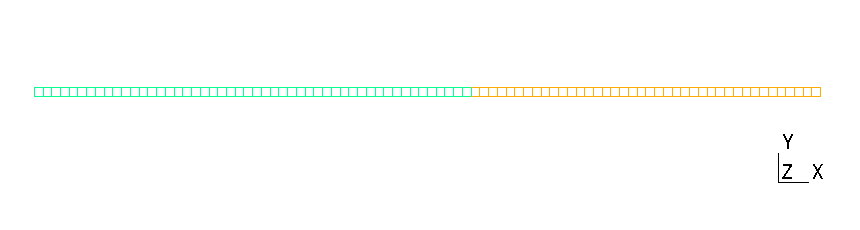
\includegraphics[scale=0.33]{images/bar_pml.png}
\caption{1D bar with medium and PML}
\label{fig:bar}
\end{figure}
\item Fixed end for the PML.
\item Input at the extremity of medium: Ricker wave.
\end{itemize}

\end{frame}

\begin{frame}{Results}

\begin{figure}
  \centering
  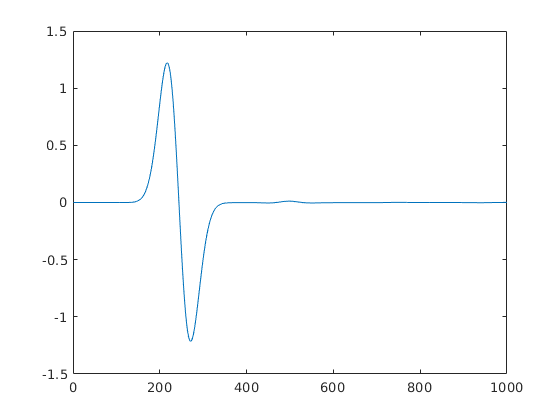
\includegraphics[width=0.47\linewidth]{images/recordingx_50.png}
  \label{fig:recx}
  \caption{Displacement recorded at the middle of the medium in x direction}
\end{figure}
\pause
\begin{itemize}
\item Very slight reflection due to the truncation interface.
\item No reflection going back in the medium from the fixed end of the PML.
\item Matlab ($8.033s$) / Akantu ($7.351s$).
\end{itemize}
\end{frame}
